% Chapter Template

\chapter{Recommendations} % Main chapter title

\label{Chapter4} % Change X to a consecutive number; for referencing this chapter elsewhere, use \ref{ChapterX}

\lhead{Chapter 4. \emph{Recommendations}} % Change X to a consecutive number; this is for the header on each page - perhaps a shortened title

A table of K-12 CS benchmarks tailored specifically for Newman can be found in Appendix \ref{AppendixNEWMAN}. These benchmarks were compiled using frameworks and curriculum from the CSTA (Appendix \ref{AppendixCSTA}), ISTE (Appendix \ref{AppendixISTE}), Computing at School (Appendix \ref{AppendixCOMP}), College Board (Section \ref{CBAP}), universities, code schools, and other online resources. \par
It felt necessary to tailor benchmarks specifically for Newman given some of the shortcomings of existing standards. CSTA benchmarks are narrowly specific in some subject areas, overly vague in others, or excessively pedantic (e.g. ``use technology to conduct age-appropriate research''). ISTE and the College Board's AP are restrictive in their sole focus on upper school. By picking from and refining established benchmarks, the list enumerated in Appendix \ref{AppendixNEWMAN} hopes to provide a concise but thorough set of standards that can be used as the bedrock framework for an aligned, K-12 CS program at Newman.
%----------------------------------------------------------------------------------------
\section{Lower School}
It is exciting to report that Media and LS science currently address the coding benchmarks outlined in Appendix \ref{AppendixNEWMAN}. The following recommendations explore potential ways improve upon the current program.\par 
Using Media time to explore physical computing may help reach a group of students that responds well to tactile instruction. Robotics also serves to introduce engineering at an early age, in addition to reinforcing CS concepts learned through online coding platforms. Hardware programming occurs in 2nd and 5th grade science through Bee-Bots or LEGO WeDo, but time with these technologies is limited and could be augmented by Media. Unfortunately, Susie Toso reports that the Media block is barely enough time to get students logged in and coding; adding hardware only complicates setup time. The need for funding or additional professional development may be another barrier to physical computing.\par
Kodable is currently one of the main online platforms used to teach coding in the LS, and so a critical evaluation of its strengths and weaknesses should inform its use in the classroom. One of the issues with Kodable is that many of the lessons follow the same format; there is little variability within units (``Loopy Lagoon,'' ``Condition Canyon,'' etc.). While repetition helps to reinforce concepts, the formulaic exercises may develop high proficiency with the game without developing a foundational understanding of the underlying skill.\par 
Another potential weakness of the platform is that it does not visually reinforce terms; the absense of text labels (``functions,'' ``loops,'', etc.) may be an intentional design decision to accommodate new readers, but developing a coding vernacular is an important step towards identifying themes and ideas across CS. On the plus side, the accompanying lesson plans are very thorough and outline solid learning objectives that teachers can use to reinforce concepts (e.g. ``functions help recycle code so there are no repeats''). That said, these teacher resources are dense and could be confusing, particularly for teachers who may be new to CS. Distilling these lesson plans down in a way that is digestible for the intended audience, K-5 students, may not be straight-forward.\par
\par
The section Asteroidia is perhaps the most problematic section, which calls into question the validity of the platform as a whole. As an experienced programmer, I struggled to determine how the exercise (shooting asteroids) was linked to a computer science concept; after reading the teacher resource, I can say that the link between shooting asteroids and variable assignment is tenuous as best. In general, I found the section to be little more than an overly complex, confusing shooting game with unclear numbers and letters, all of which were supposed to communicate variables, Strings, and Ints.\par
The important takeaway from this section, a point that is relevant to any lower school coding platform, is that the underlying concepts and learning objectives should match the age-appropriate benchmarks enumerated in Appendix \ref{AppendixNEWMAN}. Kodable tries to cover middle and upper school subjects in its K-5 platform, with mixed results. Variables (the core learning objective of the aforementioned Asteroidia section) are not a recommended benchmark until middle school because students have not explored this relatively complex subject in math classes. The same goes for Strings, Ints, arrays, and classes (subjects explored in Kodable lessons). Early exposure is certainly not detrimental, and in some cases may be advantageous, but in the case of Kodable, attempting to present advanced material resulted in a confusing asteroid game. Sticking to K-5 benchmarks is likely a better use of coding time, as additional emphasis on loops, sequences, conditional statements, and functions will lay a foundation for future advanced CS coursework.\par 
All of these criticisms aside, Kodable is still a good resources for PK-2 coding. The sections on sequencing, problem decomposition, loops, conditionals, and functions clearly communicate ideas through fun, engaging exercises. By providing additional context to help students identify recurring ideas and themes, which Susie is already doing, and exposing students to additional coding platforms (currently the case), Kodable can be considered one of several tools in the early education coding toolbox.\par
The other heavily-used platform, Code.org, currently offers a series of impressive online courses. Unlike Kodable, lessons are variegated, and there is opportunity for free play (as opposed to exercises with a single solution). The online curriculum also includes ``unplugged'' activities, activities that don't require a computer, which is another way to actively engage students in a hands-on experience of CS. In addition, the ability to ``see code'' may allow curious students to get an early taste of text-based coding, the step beyond block-based programming. Videos from diverse professionals in the field help to communicate at an early age who codes (Women! People of color!) and what coding entails.\par

Another issue that may be worth exploring is the gap in the LS CS sequence since 5th graders currently do not take Media. Since Susie Toso currently works part-time, she would not be able to cover 5th grade even if there were space in the schedule. The other gap (PK and K) is not as concerning. While coding exercises and platforms exist at this age, there are a limited number of benchmarks to be covered at the lower school level, and beginning before 1st grade may not be a valuable use of time.  \par
As illustrated in the LS faculty brainstorm (Appendix \ref{AppendixBRAIN}), there may be \textit{computer literacy} benchmarks, in addition to coding benchmarks, that should be articulated and addressed. While these topics should not necessarily be the purview of Media, establishing a list of computer literacy benchmarks to be distributed between technology, the library, and the classroom may help to ensure that students don't fall through the cracks, as well as help establish clear expectations between teachers. With the hiring of a new LS librarian, this is an opportune time to develop library curriculum that meets some of these computer literacy benchmarks. Conducting internet research, safely using the internet, and creating word processing documents could be just a few examples of important computer-related topics that do not need to take up coding time. Finally, keyboarding is another important computer literacy skill that is covered by classroom teachers. Examining the efficacy of this program (and debating the overall necessity of mandated keyboarding) should be explored by LS teachers and administrators. \par
One final recommendation is to consider a capstone coding project or assessment prior to 6th grade.  This type of project may help to ensure all students are on the same page upon entering middle school. Many online platforms offer assessment tools, but an open-ended Scratch project, for example, could be a more creative way to demonstrate mastery.\par
Oskie Creech, the coordinator of Design Thinking and Innovation at Newman, suggested the possibility of a final coding project in 5th grade. He currently sees all 5th graders for design thinking and said that one semester could be devoted to coding. Since coding lends itself nicely to open-ended design problems and since there is currently a CS gap in 5th grade, his class may be an optimal place in which to implementing a capstone coding project.\par 
\hiddensubsection{Summary}
To summarize, Susie Toso has laid a framework for coding in lower school Media, and Jennifer Williams and Elaine Sevin supplement CS content with LEGO WeDo and Bee-Bots in 2nd and 5th grade science. Thanks to the current curriculum, students are leaving lower school with an understanding of the benchmarks enumerated in \ref{AppendixNEWMAN}.\par 
Moving forward, additional programmable hardware and unplugged activities (refer to Section \ref{unplugged} for additional details), if feasible, would help to diversify the instruction. Sticking to Code.org and Scratch (as opposed to Kodable) beyond 2nd grade is recommended. Continuing to ensure that lessons provide verbal reinforcement of concepts, provide context, and draw parallels between platforms is also important (e.g. ``a function recycles code,'' ``loops repeat code---in what other programs did we see loops?''). Developing a set of computer literacy benchmarks that are distributed between technology, library, and the classroom will help to create accountability and set expectations for non-coding computer skills. And finally, exploring the idea of a capstone coding project during 5th Design Thinking would help to ensure all students are ready for CS at the middle school level.\par


\section{Middle School}
Finding a way to meet middle school CS benchmarks outlined in Appendix \ref{AppendixNEWMAN} is arguably more difficult than in other divisions, thanks to limited space for electives. In this case, integrating CS into existing courses might the easiest way to expose all students to coding. Rather than advocating for a particular implementation strategy, however, this document will explore the pros and cons of a few possibilities.\par

\hiddensubsection{CS Integration}
For a more thorough analysis of the pros and cons of CS integration, please refer to Section \ref{csint}. \par
There are innumerable possibilities for the types of projects that can be incorporated into any discipline. An easy and common integration approach is to have students develop interactive multimedia presentations (complete with sounds and moving characters) using Scratch. Example projects include animating historical events, illustrating book reports, or teaching geology lessons. Scratch gives students a creative, hands-on platform for exploring any subject with code.\par
Code.org offers middle school curriculum that uses coding as a tool to teach algebra and science. The science curriculum explores life, physical, and earth sciences. Modules include modeling and simulating ground water, ecosystems, and planetary systems using code. In the algebra lessons students design a video game and simultaneously use coding to explore order of operations, the Cartesian plane, functions, and word problems \cite{codeorgal}. The non-profit highlights one advantage of integration: ``By shifting classwork from abstract pencil-and-paper problems to a series of relevant programming problems, Code.org \textbf{CS in Algebra demonstrates how algebra applies in the real world}, using an exciting, hands-on approach to create something cool" \cite{codeorgal}.  \par
If Newman decides to take the route of integration, a series of scaffolded projects distributed between grades and subjects could help meet the benchmarks enumerated in Appendix \ref{AppendixNEWMAN}. Two projects each year (in math, science, English, art, or history) would likely be sufficient to meet these standards. An integration coordinator would likely be needed to build relationships with interested teachers, develop projects inline with existing curriculum, provide professional development, and assist in the execution of the coding projects. While there would initially be substantial work on the front-end, this approach has the potential to be more effective and robust in the long-run.  \par

Another possibility discussed this year by Peter Cline, the Head of Middle School; Lisa Swenson, the 6th grade science teacher and class dean; and Jenna deBoisblanc was the possibility of flipping Lisa's ``general'' science course into a course that strongly incorporates coding into the curriculum. ``Exploratory Design," a coding, engineering, and design thinking elective currently offered at Greenhill School in Dallas, Texas, may be a good a model the evolution of this course. From the ``Exploratory Design'' description:
\begin{blockquote} 
``This hands-on exploratory class takes a thematic approach to the presentation and solution of problems. Students are formally introduced to problem-solving processes from the fields of computer science, engineering, and science as they seek to develop products and models that address a specific set of problems. Students work with a set of guiding processes drawing from Design Thinking, Engineering and Design, Computational Thinking and Next Generation Science Processes."
\end{blockquote}
Topics include ``Mission to Mars," ``The Deep Abyss," ``Feeding the World," and ``Energy for All"---topics that explore remote sampling, remote communication, contamination, planetary geology, pressure, modeling, and renewable energy. Coding, engineering design, and design thinking are emphasized throughout the curriculum.\par
Arduinos, easily-programmable computers for creating electronics projects, could be the perfect tool to complement existing science curriculum; currently Lisa covers electricity, magnetism, geology, water, weather, and climate. Arduinos are designed to program electronics and can used to introduce electricity, simple circuits, breadboards, LEDs, voltage, current, and resistance. In addition to electricity, Arduinos are great tools for environmental science labs. \href{https://alejandroquinteros.files.wordpress.com/2012/11/environmental-monitoring-with-arduino.pdf}{``Environmental Monitoring with Arduino''} is a free, online PDF that contains projects such as ``Humidity, Temperature \& Dew Point Display'' and ``Measuring Water Conductivity.'' \href{https://publiclab.org/}{Public Lab}, a non-profit based in New Orleans and New York that develops DIY environmental sensors for communities and education, relies heavily on Arduino. Some of their ``Open Water'' sensors include Riffle Water Monitoring (open hardware device that measures some of the most common water quality parameters), and the The Homebrew Sensing Project (uses spectroscopy to indicate water contamination) \cite{publab}. These are just a few examples of projects that could be adapted to water, weather, or climate curriculum. \par 
Given the versatility of Arduinos---their ability to sense the environment, control motors, blink LEDs, generate sounds, etc.---they are a perfect prototyping tool for design thinking projects. Lisa's class currently participates in a design thinking exercise called, ``Light It Up,'' in which students develop design thinking solutions using LEDs and simple circuits. With a few lines of code, students could program Arduinos to blink, to turn on with the push of a button, to fade in response to a sliding switch, to act like a timer, to control rainbow LEDs, and so much more. A platform like Arduino could take prototypes in this design thinking project to the next level while exposing students to CS.\par
A science course with heavy integration of coding has the advantage of reaching every student in the 6th grade and giving students substantial CS exposure. This course could easily meet the middle school benchmarks in Appendix \ref{AppendixNEWMAN} while still covering environmental content, electronics concepts, and design thinking projects.\par 
Another advantage of a coding course with Arduinos is that Arduinos could serve as a perfect bridge from LS to MS, and MS to US computer science. In addition to programming Arduinos in a text-based coding language (based on C++), students may also program Arduinos in Scratch, a block-based coding platform currently used in the lower school. The ability of this platform to be used in both programming formats creates a seamless coding transition between divisions.\par
The issue of PK-12 science alignment is one major concern brought up in response to this proposed approach. Jennifer Williams, the Department Chair Lower School Science, articulated this concern: 
\begin{blockquote} ``The Lower School science portion of the curriculum adjusted our scope and sequence three years ago to pick up electricity and magnetism, so Lisa could have a more environmental, earth focus for sixth grade science. She is still teaching these concepts, since there would be a gap of four years of students not having any electricity or magnetism studies with the movement of these topics into LS. This movement of these concepts was difficult for us to absorb, since students in grades Pre-K through 4th do not have science every day of a school week. It also meant that our study of the moon had to be cut in 2nd grade to make the change for electricity. Susan also had to cut and/or shorten aspects of her program, too, for the incorporation of magnetism. While we do not mind addressing these concepts in LS, please realize that it does have effects on our tight spiral in the LS."
\end{blockquote}
Another concern with a coding-heavy 6th grade science course is that science already struggles to cover a vast amount of content, and adding coding would only exacerbate restrictions on time. Even if the ultimate objective is to preserve existing science curriculum but augment exercises and projects with coding, there may be overhead associated with teaching CS, overhead that may come at the expense of existing science content. As one MS science teacher put it, ``I have often contended that there is far more science to teach in middle school than there is time to teach science.  Why limit the science that the science department attempts to convey?" \par
This concern about coverage emanates from a more fundamental disagreement: the issue of whether computer science belongs in science at all. 
``I’m not exactly sure why the science department is the proper venue for introducing either electronics or coding into the curriculum... We actually once had a computer science department and if there seems to be a renewed interest in that arena, I’m not sure why science is the place to integrate." While this position is not universally-held among faculty (Greg Malis: ``The ultimate goal of science is to formulate hypotheses, test, and debug. That, in a nutshell, is what coding's about"), it is clear that tensions exist regarding the possibility of inserting CS into science courses (or for that matter, any existing course).\par
Considering that this concern has the potential to derail any attempts at integration, I'd like to offer a personal opinion in response to the argument that CS doesn't belong in science. I should note that the use of the first person pronoun in this paragraph is a deliberate choice that diverges from previous attempts to retain objectivity; the choice is meant to emphasize that my view is both debatable and potentially contentious.\par 
That said, of the scientists I currently know in grad school or in industry---a current physicist grad student and former classmate, my environmental science college friend who is building geology maps, my brother doing a psychology PhD at NYU, my best friend getting a PhD at MIT Media Lab, and a fellow physics major who is currently working for an engineering firm that develops drones---every single one of these scientists writes code on a regular basis either to automate testing in Matlab, analyze data with Python, or code embedded systems with C++. In my mind, the argument that programming doesn't belong in science is akin to the argument that calculators don't belong in math, or that computers don't belong in science. Coding is a tool just like Excel is a tool, just like computers and calculators are tools, all of which are used every day in science to conduct research and actively explore the world. Coding has the added benefit of being able to model complex systems virtually, to simulate the impacts of climate change or chemical reactions, to model and predict disease transmission, to illustrate and interactively manipulate the laws of physics. Coding not only has the potential to aid and accelerate the progress of science, it has the potential to improve, through models and hands-on coding projects, the experience of science education. And finally, the computational thinking mindsets associated with CS have wide-ranging benefits, including the development of better, more logical problem solvers. For these reasons, I would argue that coding is a highly-relevant, necessary practice in the modern scientific method and in science education.\par
Now, should the onus of teaching CS fall solely on the back of science? No. Nor should science blindly adopt coding without reviewing the impacts on K-12 science curriculum. Just as computers (or reading and writing for that matter) are universal tools employed and refined in all subjects, so too should coding be the responsibility of all subjects. Integration must occur with the active participation of teachers and with buy-in from department chairs to ensure cross-division content alignment is preserved. Ultimately, successful integration should augment existing content and projects in a manner that is both seamless and unobtrusive. But regardless, before CS integration can take place, it is important to understand and embrace the benefits of coding to each department and division.\par

\hiddensubsection{Art Elective}
Of the nine INDEX schools interviewed for this report, the most common way that computer science was implemented in the middle school was through the arts. Six of eight schools with middle school CS programs offered either a required or elective coding course in the arts rotation. At Greenhill School all 5th and 6th grade students take ``Exploratory Design,'' a design thinking and engineering CS course that lasts one trimester and shares an elective block with another art credit. At St. Margaret's in San Juan Capistrano, CA, 6th and 7th graders elective block is comprised of 1/4 art, 1/4 music, 1/4 health \& wellness and 1/4 CS. Winchester Thurston in Pittsburgh, PA, has a (required) one-trimester elective each year of middle school, in addition to a maker elective.\par
There are innumerable possibilities for an engaging art-themed coding course. Using Arduinos to create wearable tech LED clothing, electronic music instruments, or interactive robots are just a few examples. As discussed in the previous section, Arduinos could serve as a perfect bridge from LS to MS, and MS to US computer science because they can be programmed in a text-based coding language (based on C++) as well as with Scratch, a block-based coding platform. But regardless of the platform, coding is a very creative tool that could easily supplement the current arts rotation.\par
The most obvious advantage of offering CS through the arts rotation at Newman (a trimester, rotating sequence) is the relatively low barrier to entry; teacher buy-in is not as critical as it might be through an integrated approach. A standalone course negates the need for professional development and can be implemented almost immediately.\par
Perhaps the greatest argument against implementing CS through the arts is that students who take band, a year-long art elective, would miss out on exposure to CS. In addition, enrollment in existing performing and visual arts courses would be impacted, particularly if (as this document recommends) CS is required every year of middle school. As discussed in Section \ref{csint}, a standalone course is dependent on finding a talented CS teacher. \par

\hiddensubsection{Club/ Advisory/ Flex}
%TODO figure out advisory and flex issues?
Club time is a 30-minute, once-weekly opportunity for students to experience a non-traditional or non-academic subject. Current clubs include cooking, chess, chemistry, film, ping-pong and more. Since all middle school students take club, allocating this time block to coding has the advantage of offering CS exposure to all students in 6th-8th grades. Teachers or advisors could use online coding platforms like Code.org, platforms that require minimal teacher input in order to deliver CS curriculum. Online platforms would reduce the need for substantial, division-wide professional development to deliver instruction.\par 
When asked about the possibility of using club time for middle school-wide CS instruction, Kate Loescher, the sixth grade science teacher who previously ran the Middle School Coding Club, seemed optimistic about the idea but worried about the need for professional development. During club Kate assigned Kahn Academy exercises to students, but did not actively monitor their progress. If coding were mandatory, however, she is confident that active engagement from teachers could lead to meaningful student progress. In order to prepare for questions, Kate spent a little time working through Kahn Academy exercises. She also directed advanced students to help students with questions. It was not difficult to facilitate the club and help students through problems, but Kate pointed out that she likely has more CS exposure than the rest of the faculty. \par
One of the difficulties of club is the disjointed timing. In Maker Club, as an example, it's difficult to maintain continuity between projects given that the club meets once per week. The thirty minute time block also makes it difficult to accomplish substantial projects; reorienting and eating snack takes half of the block. The other concern is that club time may be an integral part of the Newman middle school experience. The relative merits of clubs must be considered in order to make a decision about its role the CS implementation solution.\par

Advisory time is another potential avenue for CS. Advisory meets three times a week, shares the same time block as club, and runs into similar issues: short blocks and the potential to displace an important middle school experience.   \par
Another possibility is to do coding during flex time. All grades in 6th-8th have flex during the same block as PE but on alternating days. Flex has the advantage of meeting more regularly (every other school day), of meeting for 45 minutes instead of 30, and for splitting up each grade into a different time block. The advantage of a separate time blocks is that it might enable one CS subject-matter expert to attend multiple classes throughout the day in order to support teachers and students. \par
The problem with using flex time for CS, however, is that this time block is currently used by students to get extra help or work on homework. Repurposing this time may not be to the advantage of students, particularly those who are falling behind. If, however, the only requirement is that students finish a particular online coding unit (a self-paced but teacher-tracked unit) before the end of the trimester, students may be able to spend time coding when other assignments are light and vice versa. In addition, meeting the Newman benchmarks in Appendix \ref{AppendixNEWMAN} may only take an equivalent of a trimester worth of flex time, a potentially manageable burden when spread throughout the year. \par 
In any of these solutions, substantial analysis and input from teachers, students, and administrators will be necessary before moving forward. Professional development will be necessary to ensure that teachers feel comfortable with CS instruction since they would be required to teach, or at the very least, monitor student progress. Developing or executing highly-engaging CS exercises may also be more difficult since the teachers implementing the projects will not be subject-matter experts. There are a variety of online programs, however, that offer fun, engaging coding experiences, in addition to providing student tracking and online assessments (refer to Appendix \ref{AppendixTools}). 

\hiddensubsection{A Path Forward...}
Taking a middle school CS program from zero to sixty is neither advisable nor possible; instead, small, easy-to-prototype projects that gradually build teacher support and interest are the appropriate path forward. To that end, working with early adopters to integrate a few easy, unobtrusive coding projects into existing curriculum at each grade level should be the focus next year. Lisa Swenson has already expressed interest in implementing coding in her classroom, and as discussed in previous sections, design thinking projects like ``Light It Up'' may be the perfect avenue for coding with Arduinos. Scratch multimedia presentations that can replace PowerPoint are another example of an easy introduction to CS integration. With a few successful projects under the belt, discussions may evolve about how to offer CS in a more substantial way that meets the benchmarks in Appendix \ref{AppendixNEWMAN}, either through a standalone course or through integration. In any scenario, however, a knowledgeable coding advocate will be necessary to keep the ball rolling, to educate teachers about CS, and to help develop coding projects.

\section{Upper School}
Unlike the middle school schedule, the upper uchool sequence affords time and space for computer science electives. The rotating eight block schedule means there are 32 possible credits, although Newman students rarely graduate with greater than 28. The student handbook stipulates that students must complete 24 academic credits to graduate (refer to Table \ref{tab:usreqs}). \par

\begin{table}
	\begin{center}
\begin{tabular}{ | l | c | }
	
	\hline
	\textbf{Subject} & \textbf{Credits} \\ \hline
	English & 4 \\ \hline
	Mathematics & 4 \\ \hline
	History/Social Studies & 4 \\ \hline
	Science & 3 \\ \hline
	World Languages & 3 \\ \hline
	Arts & 2 \\ \hline
	Physical Education & 2 \\ \hline
	Electives & 2 \\ \hline
	\textbf{Total} & \textbf{24} \\ \hline
\end{tabular} 
\caption{Upper School Graduation Requirements} \label{tab:usreqs} 
\end{center}
\end{table}
\par
The elective space (two required elective graduation credits) is one possible avenue for CS courses, as is the Art Department. Offering CS courses with titles like, ``Creative Coding'' or ``Virtual Reality Animation'' may allow courses to fit into the arts rotation. Offering coding courses as arts electives may attract a broader audience, particularly girls, than traditional CS electives. The perception of arts courses as less rigorous than science electives (for better or for worse) may also encourage greater participation. On the other hand, offering coding through the Art Department may impact the enrollment of other art courses, particularly if a variety of CS electives are implemented. Since many students choose to take art courses to fill the two credit additional elective requirement, however, the impact on existing art classes may be the same regardless of whether CS is offered as a general elective or an art elective. Nevertheless, finding the appropriate home for computer science---in art, science, or math---should be discussed by teachers and administrators.   \par


\hiddensubsection{1st Tier}
As a first step, implementing an introductory CS elective with broad appeal is paramount. There are many different possible introductory courses in a variety of different programming languages, but the priority of this course must be to hook students. Highly-engaging, fun, hands-on, and topical projects should communicate foundational concepts outlined in Appendix \ref{AppendixNEWMAN}. Students should leave the class understanding the broad applicability of CS, as well as the potential for innovation and creativity in a multitude of fields. \par
One possible introductory course, The Art of Making, is outlined in Appendix \ref{AppendixCC}. This hands-on course strongly emphasizes coding, but also teaching fundamentals in 3D printing, laser cutting, and electronics. The course relies on Processing, a visual programming language designed for artists, and Arduino, a programmable platform for interactive electronics projects. By leveraging these tools together, the possibilities are only limited by the imagination: LED dresses that sparkle when an accelerometer registers movement, drones, electronic music instruments, interactive data visualizations, and so much more. \par

\hiddensubsection{2nd Tier}
There are already students at Newman who are ready for a second tier CS course. A course titled ``Creative Coding'' (outlined in Appendix \ref{AppendixCC}) could offer the same creative freedom as the introductory course but with advanced, second tier topics (enumerated in Appendix \ref{AppendixNEWMAN}). In addition to the previous benchmarks from tier one, tier two introduces object-oriented programming structures (either classes or prototypes depending on the language). \par

While this document strongly recommends against offering AP Computer Science A, at least in the early stages of CS, Creative Coding lends itself nicely to the new AP CS Principles framework (for a full discussion of the benefits and drawbacks of teaching each AP CS course, please refer to Section \ref{proconap}). AP Computer Science Principles (the new course) may offer both the national recognition of an AP while still preserving the creative and innovative component of CS. This AP is young, so time and experimentation may be necessary to determine the course's true value.\par 
One requirement of offering the AP is that the course be year-long in order to adequately prepare students for the exam. The benchmarks outlined in Appendix \ref{AppendixNEWMAN} could be covered in a single semester. An AP CS Principles course should cover the benchmarks listed in tiers two and three. If a year-long course at the second tier is not possible or advisable, the AP could be offered as a third tier course.\par

\hiddensubsection{3rd/4th Tier}
A third tier of CS electives will ensure that motivated students can continue to develop as computer scientists. There are infinite possibilities for courses that can meet the advanced benchmarks in Appendix \ref{AppendixNEWMAN}. Future courses will likely depend on the instructor, student preferences, and total enrollment. Like Creative Coding, any of the courses listed below could likely be adapted to the AP CS Principles framework. These course titles could also be used as a fourth tier by ensuring content and projects meet the benchmarks listed in Appendix \ref{AppendixNEWMAN}. Potential titles include:
\begin{itemize}
	\item Web Design and Development
	\item Software Engineering
	\item Mobile Apps
	\item Robotics with Python
	\item Virtual Reality with JavaScript
	\item Advanced Physical Computing
\end{itemize}
Absent from this list are courses titled, ``Advanced Data Structures,'' ``AP CS A,'' and ``Object Oriented Programming Using C++''---courses currently taught at other high schools that fail to relate CS to other disciplines, that emphasize CS theory without making room for creative expression, and that, at least historically, have failed to reach a broad, diverse audience. Creative, open-ended, project-driven courses that teach equivalent computational thinking concepts should comprise 3rd and 4th tier CS. \par

\hiddensubsection{Innovation Ecosystem} 
Section \ref{innovate} makes an argument for the incorporation of CS into curriculum that focuses on design, engineering, making, and innovation. The tools and technology of Newman's Makerspace are the perfect venue for exploring innovation through code. This track system begins with The Art of Making (refer to Appendix \ref{AppendixCC} for a sample syllabus), which serves as the introduction to coding, design thinking, 3D printing, laser cutting, and electronics---the foundation of all courses to evolve out of the Makerspace. \par
At the next level students may choose between two tracks: computer science or engineering design. Each track may comprise of scaffolded tiers of courses. Although the tracks emphasize one particular discipline over the other, both tracks continue to expose students to coding, design thinking, and engineering design.\par
\par
\begin{figure}[!ht]
  \caption{Innovation Ecosystem}
  \centering{
    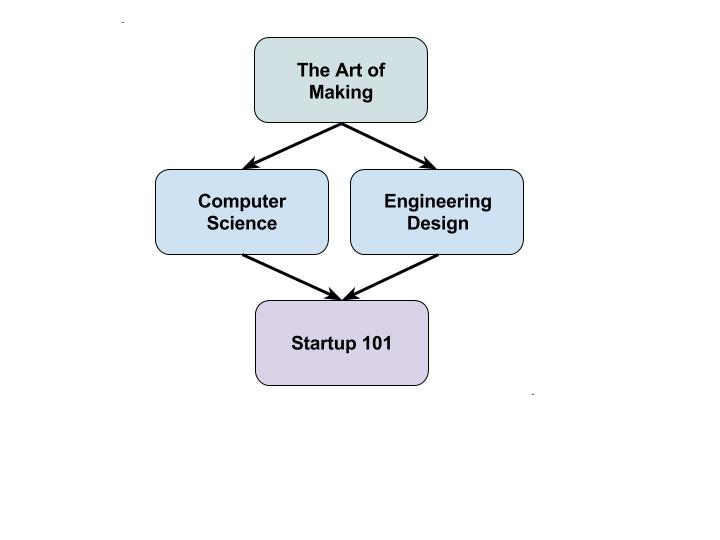
\includegraphics[scale=.5]{CSTiers2.jpg}}
\end{figure}

Potential courses in each track are outlined below.\par
Computer Science
\begin{enumerate}
	\item Creative Coding
	\item Web Design and Development
	\item Software Engineering
\end{enumerate}
Engineering Design
\begin{enumerate}
	\item 3D Art and Design / Tech Theater / Environmental Engineering Design 
	\item Industrial Design
	\item Robotic Systems
\end{enumerate}	

Finally, the tracks reconverge with Startup 101, a course focusing on the ideation, creation, testing, and marketing of unique products and services. The course builds on skills acquired in computer science, engineering, 3D modeling, and design, but adds the element of entrepreneurship. Students will write business models and develop marketing strategies. By the end of the course, students will have an understanding of pathways to innovation, in addition to an understanding of how successful products are launched.\par

\hiddensubsection{Required Exposure}
This document strongly recommends that the Upper School adopt a 1/2 credit CS graduation requirement. A mandated credit, as opposed to an optional elective, ensures that every student---especially groups typically underrepresented in CS---get exposure to coding prior to college. The importance of CS and the dire need for coding experience is explored in Chapter \ref{Introduction}. Of the nine INDEX schools interviewed about CS, the three schools with the most impressive CS programs all had graduation requirements of approximately one semester (refer to Section \ref{index}).\par
That said, there are a few potential problems associated with a graduation requirement. Mandated credits in the Upper School are currently impacting scheduling for certain students; additional requirements would place even greater restrictions on the courses students can take. In addition, a graduation requirement would necessitate the hiring of additional faculty to teach CS courses, which may prove to be difficult. Staffing difficulties, however, should not prevent the enactment of a graduation requirement. The ubiquity of professional development opportunities and online resources should enable non-CS teachers (possibly math or science) to pick up a language. Hiring and training a new teacher, however, may take time.\par
If a required graduation credit is not feasible within a reasonable timeline, mandating CS integration in the Upper School should be considered. Re Each department could be required to expose students to CS through a project at some point during 9th-12th grade, or class deans could be responsible for ensuring that at least one course exposes students to CS each year. Ideally these coding experiences would be scaffolded or coordinated in such a way that students still meet the minimum CS requirements outlined in Appendix \ref{AppendixNEWMAN}. An integration coordinator would be necessary to help non-CS teachers brainstorm and implement project ideas, coordinate between departments and classes to ensure that each class gets necessary exposure to coding, and develop content that meets necessary graduation requirements.\par
The drawbacks and benefits of CS integration are explored in more depth in Section \ref{csint}. One of the primary drawbacks of integration is placing additional burdens on upper school teachers who are already struggling to meeting curriculum requirements. The lack of understanding of CS and the need for professional development is another primary drawback. A integration coordinator, however, may help to mitigate both of these obstacles and would allow all students to get CS exposure without requiring additional graduation requirements.\par

\hiddensubsection{Online Education}
For a full analysis of online platforms, their merits and shortcomings, please refer to \ref{procononline}.\par
There are several examples where online programs add clear value to Newman's CS offerings. Allowing platforms like Global Online Academy or CodeHS to fill niche needs---such as allowing self-directed students to take specific upper level courses---is cost-effective and grants students more options. In addition, using Kahn Academy or other online resources in blended classrooms as a crutch or supplement may bolster in-class instruction.\par
This document, however, does not recommend the strict reliance on online CS platforms, especially for meeting a potential graduation requirement. By the very nature of being ``cookie cutter'' and purely virtual, online platforms cannot offer the same ``rigor and relationships'' as curriculum spearheaded by a teacher. Hooking students, inspiring students, communicating the importance and broad applicability of CS, and ensuring that students recognize the creative and innovative potential of coding---these must be the priorities of a CS program at Newman. CS courses will not compete with other disciplines at Newman without the enthusiasm and relationships created by and with teachers, the personally-relevant curated projects, or the face-to-face communication. In short: Newman is known for its top-notch pedagogy; CS, a critically important field in the 21st century, cannot be the exception. \par
All of that said, hooking students is the priority, after which students may want more freedom to explore advanced topics on their own. Using online CS programs as a second or third tier course may be advisable, but only if resources or hiring difficulties prohibit an in-person CS experience. \par  

\hiddensubsection{Next Steps}
Next year two new courses will be offered in the Makerspace---``The Art of Making'' and ``Creative Coding''---which will lay the groundwork for potential upper school courses in engineering and computer science. Offering these courses as art electives to a small group of students will give time to prototype projects and give insight into the best type of CS instruction that meets the Newman CS benchmarks outlined in \ref{AppendixNEWMAN}. In time, questions related to graduation requirements, additional courses and tiers, offering the AP, and hiring/ staffing needs can be addressed. For now, drumming up student interest and building teacher support is paramount in order to build a sustainable and resilient program.
